\documentclass[border=10pt]{standalone}
\usepackage{tikz}
\usetikzlibrary{shapes,arrows,positioning,calc}

\begin{document}
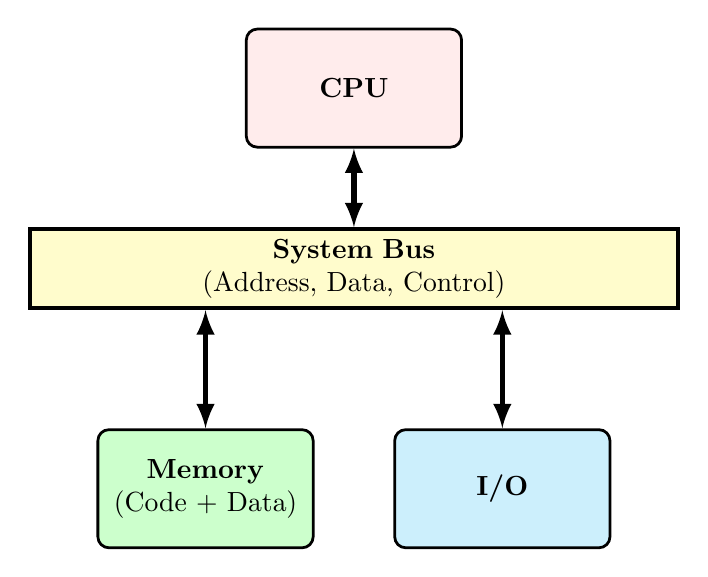
\begin{tikzpicture}[
    node distance=1.5cm,
    block/.style={rectangle, draw, fill=blue!10, text width=2.5cm, text centered, rounded corners, minimum height=1.5cm, line width=1pt},
    bus/.style={rectangle, draw, fill=yellow!20, text width=8cm, text centered, minimum height=1cm, line width=1.5pt},
    line/.style={draw, line width=2pt, <->, >=latex}
]

% Nodes
\node [block, fill=pink!30] (cpu) {\textbf{CPU}};
\node [bus, below=1cm of cpu] (bus) {\textbf{System Bus}\\(Address, Data, Control)};
\node [block, fill=green!20, below left=1.5cm and 0.5cm of bus.south] (mem) {\textbf{Memory}\\(Code + Data)};
\node [block, fill=cyan!20, below right=1.5cm and 0.5cm of bus.south] (io) {\textbf{I/O}};

% Connections - calculated for straight vertical lines
% CPU to Bus
\draw [line] (cpu) -- (cpu |- bus.north);

% Bus to Memory
\draw [line] (mem) -- (mem |- bus.south);

% Bus to I/O
\draw [line] (io) -- (io |- bus.south);

\end{tikzpicture}
\end{document}
